\chapter{Introduction} \label{chap:introduction}

Even just a hundred years ago, traffic consisted almost entirely of livestock, wagons, and pedestrians. Roads were not smooth, and little care was put into their upkeep, let alone the management of traffic. Nowadays, it is a different story. The rise of the internal combustion engine has changed how traffic has had to be dealt with, and so the rules of the road have been forced to evolve. Pedestrians are one of the few features that remain constant, yet are one of the groups most likely to deal with trouble on the road, especially when they are not being mindful of their surroundings. With this in mind, the `Danger Zone' project was born. The initial plan was to model the three basic modes of transport seen around Amsterdam – cars, bicycles, and pedestrians – using an approach combining ideas of swarm dynamics and free agent systems. This model would then be used to simulate what happens when these entities share a space. Due to difficulties faced in implementing this, however, bicycles were removed from the final iterations, and we chose an approach more closely resembling the concepts found in cellular automata.

Some studies and real-world examples\cite{hamilton2008}\cite{clarke2006}\cite{kruyswijk2016} have shown that having all traffic use the same area of pavement can actually improve safety and efficiency by forcing each individual to be much more conscious of those around them. Our `Danger Zone' model explores this problem area, examining how road vehicles interact, and allowing us to take note of any effects on traffic flow. We predict that such a shared space will improve traffic efficiency over a more traditional layout. Implications of our model include that it could also allow the testing of specific conditions that are difficult to achieve in reality (such as a sudden influx of tourists or rush hour traffic).

\begin{figure}[h]
    \centering
    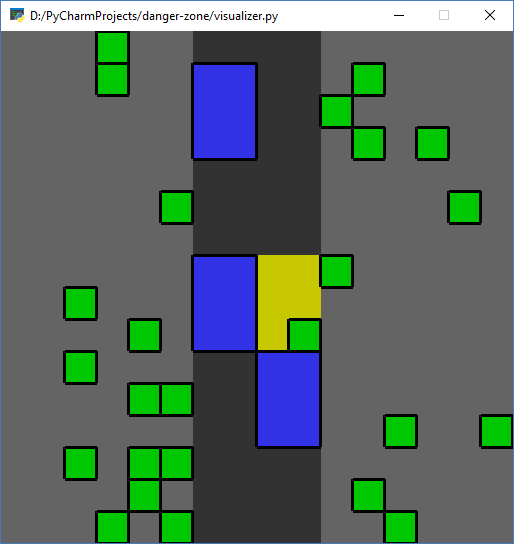
\includegraphics[width=3.3in]{images/screenshot-discrete.png}
    \caption{Screenshot of the trace playback functionality of the second iteration of the simulator.}
    \label{fig:screenshot-discrete}
\end{figure}
